\documentclass[12pt]{amsart}
\usepackage[margin = 4cm]{geometry}
\usepackage[utf8]{inputenc}
\usepackage[usefamily=sage]{pythontex} 
\usepackage{colortbl} 
\usepackage{xcolor}
\usepackage{tikz}

\newtheorem{ejer}{Ejercicio}

\title{Tarea 6. Bases}
\author{Manu}

\def\r{\mathbb{R}}

\begin{document}
\maketitle

\begin{ejer} 
Sea la aplicación $f: \r ^2\to \r ^2$ tal que 
\[ M_{B'B}(f) = \left[ \begin{array}{rr} -2 & 2 \\  -1 & 1 \end{array} \right], \]  siendo $B'$ y $B$ las bases dadas por las matrices 
\[ B' = \left[ \begin{array}{rr} 6 & -5\\ 5 & -4 \end{array} \right] \ \hbox{y} \ B = \left[ \begin{array}{rr} -1 & -5\\ 2 & 9  \end{array} \right].  \] Calcula $M(f)$.

Para resolver el problema puedes usar el siguiente esquema de diagrama:


$$
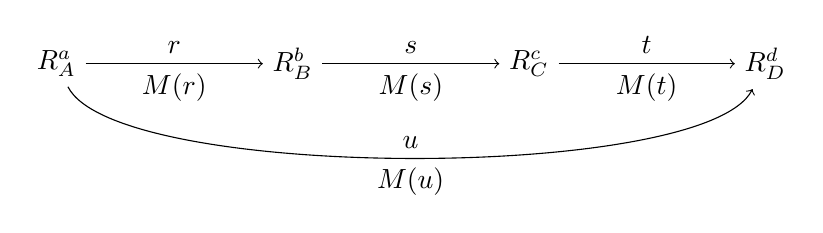
\begin{tikzpicture}[xscale = 1.5]
\node (A) at (0,0) {$\r^a_A$};
\node (B) at (2,0) {$\r^b_B$};
\node (C)  at (4,0) {$\r^c_C$};
\node (D) at (6,0) {$\r^d_D$};
\draw[->] (A) to node [above] {$r$} 
                   node [below] {$M(r)$} (B);
\draw[->] (B) to node [above] {$s$} 
                   node [below] {$M(s)$} (C); 
\draw[->] (C)  to node [above] {$t$} 
                   node [below] {$M(t)$} (D);
\draw[->] (A) .. controls (0.5,-1.5) and (5.5,-1.5) .. 
                node [below] {$M(u)$} 
                node [above] {$u$} (D);
\end{tikzpicture}
$$


\end{ejer}

{\it Soluci\'on:}
% Escribe tu Solución para el Ejercicio 1.
\begin{sageblock}
MBpB = matrix(QQ, [[-2, 2], [-1, 1]])
Bp = matrix(QQ, [[6, -5], [5, -4]])
B = matrix(QQ, [[-1, -5], [2, 9]])
BpB = Bp * B
Bi = B.inverse()
M = Bi * BpB * Bp
\end{sageblock}

Multiplicamos B' y B para obtener
$$ \sage{Bp} * \sage{B} = \sage{BpB} $$
Luego invertimos B
$$ \sage{B} \to \sage{Bi} $$
Multiplicamos B inversa, B', B y B'
$$ \sage{Bi} * \sage{Bp} * \sage{B} * \sage{Bp} \to \sage{M} $$
% Fin del ejercicio.

\end{document}
